\documentclass[final,5p,times]{elsarticle}

\usepackage{amsmath,amssymb}
\usepackage{booktabs}
\usepackage{graphicx}
\usepackage{hyperref}
\urlstyle{same}
\renewcommand{\UrlFont}{\rmfamily}
\DeclareUrlCommand\url{\def\UrlFont{\rmfamily}}
\DeclareUrlCommand\path{\def\UrlFont{\rmfamily}}
\hypersetup{hidelinks}

\journal{Pattern Recognition Letters}

\begin{document}

\begin{frontmatter}

\title{Sparse farther-sighted trees can improve forest accuracy--time tradeoffs}

\author[1]{Mathias Valla\corref{cor1}}
\cortext[cor1]{Corresponding author.}
\affiliation[1]{
  organization={Chaire DIALog, Institut Louis Bachelier},
  city={Paris},
  country={France}
}

\begin{abstract}
Decision trees are induced by a sequence of local split decisions, although the value of a split depends on the descendants it enables. We study $k$-sighted induction, a bounded non-greedy compromise between CART-style recursion and globally optimal tree search: candidate axis-aligned splits are scored by the impurity reduction achieved after a depth-$k$ local subtree is optimized. The question is practical rather than existential: does this additional sight materially improve shallow trees and bootstrap forests once fitting time is considered? On 67 PMLB classification datasets, uniform $k=2$ and $k=3$ induction improves mean accuracy over greedy $k=1$, but by small and uneven margins relative to cost. For single trees, mean accuracy rises from 0.6931 to 0.7100 and 0.7145, while mean fitting time rises from 0.0076 s to 0.3727 s and 70.90 s. For 100-tree bootstrap forests, mean accuracy rises from 0.7068 to 0.7125 and 0.7260, while mean fitting time rises from 0.0188 s to 0.6940 s and 96.19 s. A 57-dataset mixed-forest study gives the constructive exception: injecting a small number of $k=2$ trees can move a mostly greedy ensemble to a better accuracy--time point. Within a 0.7 s fitting-time budget, a 20-tree $\bar{k}=1.25$ forest attains 0.7412 mean accuracy, above lower-sight forests at comparable times. Thus one split at a time remains a strong default for single trees and uniform forests, but sparse farther sight inside forests can be useful.
\end{abstract}

\begin{keyword}
Decision trees \sep Random forests \sep Greedy algorithms \sep $k$-sighted induction \sep Optimal trees \sep PMLB
\end{keyword}

\end{frontmatter}

\section{Introduction}

Most decision-tree learners make one split decision at a time. At each internal node, CART-style induction selects the split that best improves an impurity criterion, then repeats the same operation independently in the child nodes \cite{breiman1984cart,quinlan1986induction}. This greedy rule is fast, stable enough to be useful, and still central to bagging and random forests \cite{breiman1996bagging,breiman2001random}. It is also myopic: a split is useful because of the subtree it permits, and the locally best split need not be the best first step toward a shallow predictive tree.

This paper asks when bounded non-greediness is worth its computational price. A $k$-sighted tree evaluates a candidate split by optimizing a local descendant subtree of depth $k$, then chooses the root split of the best such local subtree. The case $k=1$ is ordinary greedy induction. Larger $k$ occupies a middle ground between cheap greedy recursion and exact optimal decision-tree search.

Our question is deliberately narrow and empirical: does multi-step split optimization materially improve shallow decision trees and bootstrap forests when predictive accuracy and fitting time are evaluated jointly? The answer separates two regimes. Giving every tree more sight is usually expensive for a thin and uneven accuracy gain. In contrast, mixed forests reveal a useful compromise: a small minority of farther-sighted trees can improve the accuracy--time frontier of an otherwise greedy ensemble. The main contribution is a compact benchmark, accompanied by open code and retained result tables, that distinguishes uniformly non-greedy induction from sparse non-greedy ensemble design.

\section{Related work}

Greedy top-down tree induction was established by ID3, CART, and related algorithms \cite{quinlan1986induction,breiman1984cart}. Ensembles such as bagging and random forests reduce the variance of greedy trees by averaging many fitted trees \cite{breiman1996bagging,breiman2001random}, but the split decisions inside each tree remain local. This matters for $k$-sighted forests because additional computation can be spent either inside each split decision or on more trees.

Non-greedy decision-tree induction has a long history. Norton \cite{norton1989generating} considered downstream tree quality during induction, while Ragavan and Rendell \cite{ragavan1993lookahead} studied descendant-aware feature construction. Murthy and Salzberg \cite{murthy1995lookahead} warned that even one additional generation of lookahead can be expensive and need not improve accuracy, a theme later analyzed by Elomaa and Malinen \cite{elomaa2005lookahead}. Esmeir and Markovitch \cite{esmeir2007anytime} cast tree induction as an anytime procedure in which extra computation should be justified by better trees. Norouzi et al. \cite{norouzi2015efficient} also studied non-greedy tree optimization, emphasizing that non-greediness can enter either split selection or subsequent tree-parameter optimization.

At the other end of the spectrum, optimal-tree methods search directly over tree structures. Hyafil and Rivest \cite{hyafil1976constructing} showed that optimal binary decision-tree construction is NP-complete. Modern mixed-integer, dynamic-programming, and branch-and-bound methods have made optimal trees practical in selected regimes \cite{bertsimas2017optimal,verwer2019learning,hu2019optimal,lin2020generalized,aghaei2025strong}, but scalability remains a central limitation. The $k$-sighted rule is therefore an intermediate strategy: spend more computation locally, without committing to global tree optimization.

\section{\texorpdfstring{$k$}{k}-sighted induction}

Let $S$ denote the samples reaching a node, let $I(S)$ be the node impurity, and let $\mathcal{T}_k(s,S)$ be the frontier leaves obtained after applying candidate split $s$ and then optimizing descendant split choices for at most $k-1$ additional generations. A $k$-sighted split maximizes
\begin{equation}
G_k(s;S) =
I(S) -
\sum_{L \in \mathcal{T}_k(s,S)}
\frac{|L|}{|S|} I(L).
\label{eq:sighted}
\end{equation}
For $k=1$, this is the usual immediate impurity gain. For $k=2$ or $k=3$, the current split is chosen according to the best bounded descendant subtree it enables.

This can correct myopic split choices, but it changes the computation sharply. If $m$ split candidates are available at each internal node, a full depth-$k$ binary local subtree has a naive split-configuration count of order $m^{2^k-1}$. Implementations can cache work and stop early at pure or infeasible nodes, but the qualitative pressure remains: sight depth increases search cost much faster than it increases final tree depth.

To compare accuracy and time, we use a simple utility heuristic. Let $A(k)$ and $T(k)$ be the mean accuracy and mean fitting time at sight depth $k$. For a user who values accuracy but penalizes multiplicative increases in fitting time, define
\begin{equation}
U_\lambda(k)=A(k)-\lambda \log\{T(k)/T(1)\},
\label{eq:utility}
\end{equation}
where $\lambda$ is the accuracy penalty assigned to one natural-log unit of extra fitting time. A larger sight depth beats the greedy baseline under this utility only if
\begin{equation}
A(k)-A(1) > \lambda \log\{T(k)/T(1)\}.
\end{equation}
The break-even value $\lambda^\star_k=[A(k)-A(1)]/\log\{T(k)/T(1)\}$ is not a full decision model, but it gives a concise accuracy-time scale.

\section{Experiments}

We evaluated sight depths $k\in\{1,2,3\}$ for a decision-tree classifier and a bootstrap forest classifier on 67 PMLB classification datasets \cite{olson2017pmlb}. The protocol used one train--test split per dataset: test size $0.25$, random state $0$, stratification when possible, maximum tree depth $3$, all features available at each split, and no explicit cap on split candidates. This is a screening benchmark rather than a full model-selection study: we did not tune hyperparameters or repeat resampling. The main forest benchmark used 100 bootstrap trees with the same $k$-sighted rule inside every tree; because all features were considered at each split, the comparison isolates sight depth rather than random feature subsampling.

We then studied mixed bootstrap forests on a 57-dataset PMLB sample. Each mixed forest contains proportions $p_j$ of trees with integer sight depths $k_j$, summarized by an effective sight depth
\[
\bar{k}=\sum_j p_j k_j .
\]
This shorthand is descriptive: for example, a 90\% $k=1$ and 10\% $k=2$ forest and a 95\% $k=1$ and 5\% $k=3$ forest both have $\bar{k}=1.10$, but very different costs. We evaluated all curves at 20, 40, 60, 100, and 200 trees.

The implementation, benchmark scripts, and retained result tables are available at \href{https://github.com/MathiasValla/non-greedy-decision-trees}{https://github.com/MathiasValla/non-greedy-decision-trees}.

\section{Results}

Table~\ref{tab:aggregate} gives the aggregate benchmark. Extra sight improves mean accuracy, but the improvement is thin relative to the time increase. For single trees, $k=2$ adds 1.69 percentage points over $k=1$ while fitting time is about 49 times larger; $k=3$ adds 2.15 points while fitting time is about $9.4\times 10^3$ times larger. For bootstrap forests, $k=2$ adds 0.57 points at about 37 times the fitting time, and $k=3$ adds 1.92 points at about $5.1\times 10^3$ times the fitting time.

\begin{table}[t]
\centering
\caption{Aggregate performance over 67 PMLB classification datasets.}
\label{tab:aggregate}
\begin{tabular}{@{}lrrrr@{}}
\toprule
Estimator & $k$ & Mean acc. & Median acc. & Mean fit (s)\\
\midrule
Decision tree & 1 & 0.6931 & 0.7554 & 0.0076\\
Decision tree & 2 & 0.7100 & 0.7222 & 0.3727\\
Decision tree & 3 & 0.7145 & 0.7333 & 70.9025\\
Bootstrap forest & 1 & 0.7068 & 0.7500 & 0.0188\\
Bootstrap forest & 2 & 0.7125 & 0.7407 & 0.6940\\
Bootstrap forest & 3 & 0.7260 & 0.7612 & 96.1864\\
\bottomrule
\end{tabular}
\end{table}

Figure~\ref{fig:accuracy_time} shows the same pattern visually. Accuracy grows mildly as $k$ increases, while fitting time grows on a logarithmic scale. The break-even $\lambda^\star_k$ values are 0.00435 for tree $k=2$ versus $k=1$, 0.00235 for tree $k=3$ versus $k=1$, 0.00158 for forest $k=2$ versus $k=1$, and 0.00225 for forest $k=3$ versus $k=1$. Thus any time penalty larger than roughly 0.16--0.44 accuracy percentage points per natural-log unit of fitting time would favor greedy induction in these aggregate comparisons.

\begin{figure*}[t]
\centering
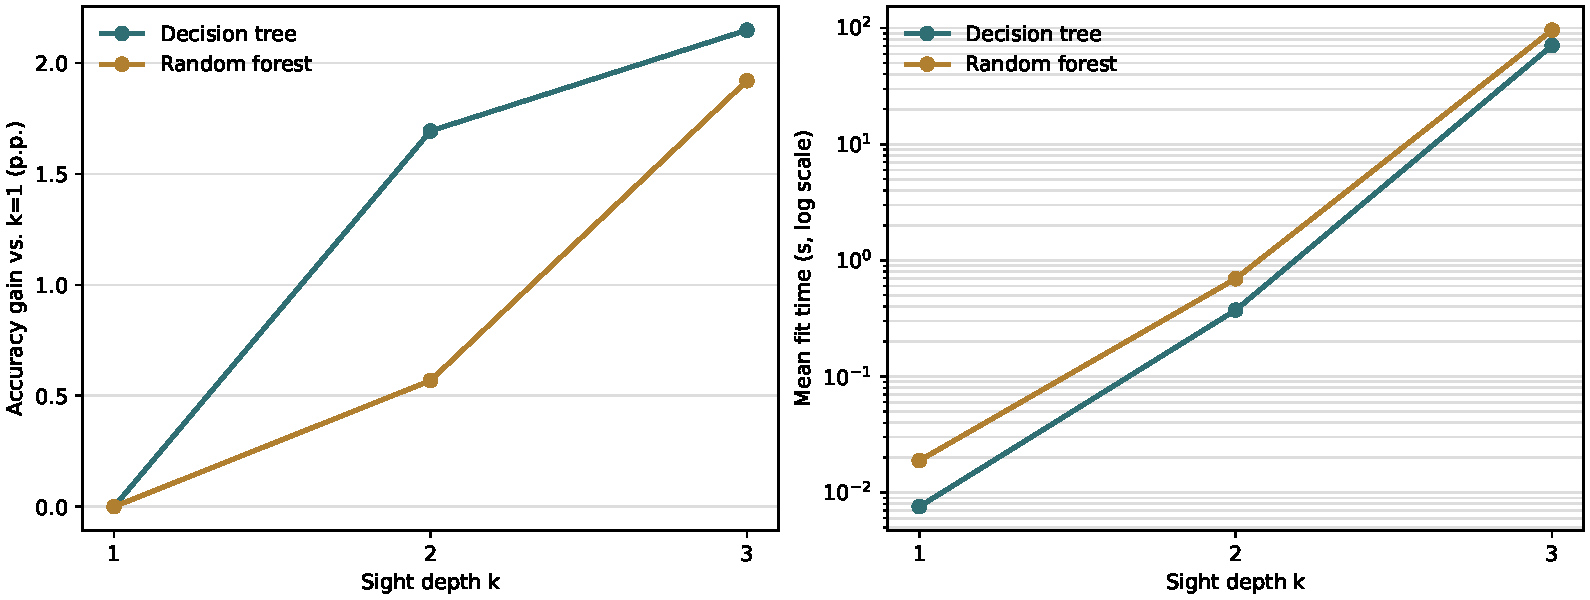
\includegraphics[width=0.86\textwidth]{Fig1_accuracy_time.pdf}
\caption{Mean accuracy gain and mean fitting time as sight depth increases from $k=1$ to $k=3$. Accuracy gains are measured relative to the greedy $k=1$ baseline.}
\label{fig:accuracy_time}
\end{figure*}

The gains are not uniform across datasets. Counting ties as wins, $k=1$ was tied for the best single-tree accuracy on 30 datasets, $k=2$ on 31 datasets, and $k=3$ on 37 datasets. For forests, the corresponding counts were 36, 29, and 29. These descriptive counts are not significance tests; they reinforce the central point that larger $k$ can alter the average, but it does not dominate greedy splitting.

\subsection{Mixed forests}

Figure~\ref{fig:forest_size} shows the full forest-size grid: the left panel plots mean accuracy against the number of trees, and the right panel plots the same grid against mean fitting time on a log scale. The grid asks whether a mostly greedy forest benefits from a few farther-sighted trees. It shows a limited benefit rather than a shortcut: $k=2$ minorities often improve the mean, but the improvement follows the same accuracy-time frontier. At 100 trees, the greedy forest has mean accuracy 0.7241 and mean fitting time 0.453 s. Replacing 5\%, 10\%, 25\%, and 50\% of trees by $k=2$ trees raises mean accuracy to 0.7346, 0.7363, 0.7458, and 0.7504, while increasing mean fitting time by factors of 2.3, 3.5, 7.3, and 13.6. A pure $k=2$ 100-tree forest reaches 0.7536 accuracy at 26.2 times the greedy fitting time.

\begin{figure*}[t]
\centering

\includegraphics[width=\textwidth]{Fig2_forest_size.pdf}
\caption{Forest-size grid for pure and mixed $k$-sighted bootstrap forests on the 57-dataset mixed-forest benchmark. Left: mean accuracy versus number of trees. Right: the same curve points versus mean fitting time on a logarithmic scale; the dashed vertical line marks a 0.7 s fitting-time budget. Each curve is evaluated at 20, 40, 60, 100, and 200 trees. Legend labels use effective sight $\bar{k}$, the average tree sight depth in the ensemble; the two $\bar{k}=1.10$ curves are distinct mixtures, one with 90\% $k=1$ and 10\% $k=2$ trees and one with 95\% $k=1$ and 5\% $k=3$ trees.}
\label{fig:forest_size}
\end{figure*}

The right panel also shows why mixed forests can be beneficial. The dashed vertical line marks a 0.7 s fitting-time budget. Within that budget, the 20-tree $\bar{k}=1.25$ forest reaches 0.7412 mean accuracy in 0.661 s. Lower-sight forests at comparable times are less accurate: for instance, the 40-tree $\bar{k}=1.10$ forest reaches 0.7368 accuracy in 0.638 s, and the 60-tree $\bar{k}=1.05$ forest reaches 0.7340 accuracy in 0.614 s. This vertical comparison is not a formal dominance result or a tuned Pareto frontier, but it is the clearest empirical case for heterogeneous sight in this grid: at comparable fitting time, replacing a modest number of greedy trees by $k=2$ trees can be better than spending the same budget only on additional low-sight trees. Thus the practical question is not only whether every tree should be farther-sighted. A small number of $k=2$ trees can sometimes move an otherwise greedy ensemble to a better accuracy--time point.

Adding $k=3$ trees is much more expensive. At 100 trees, a 95\% $k=1$ and 5\% $k=3$ forest reaches 0.7325 accuracy but costs 110 times the 100-tree greedy forest. A 95\% $k=2$ and 5\% $k=3$ forest reaches 0.7540 accuracy but costs 134 times the greedy forest. Within the evaluated grid, increasing the number of greedy trees alone does not close the gap on this sample: a 200-tree greedy forest has mean accuracy 0.7242, essentially unchanged from the 100-tree greedy forest, whereas a 20-tree $k=2$ forest reaches 0.7491 at 5.2 times the 100-tree greedy fitting time. The pure $k=3$ curve is still farther to the right and does not dominate the $k=2$ frontier. The lesson is not that greedy trees always suffice. It is that improvements from extra sight arrive through a visible and expensive accuracy-time frontier, not through a nearly free ensemble effect.

\section{Discussion}

The empirical message is conservative but not purely negative. $k$-sighted induction is a plausible correction to greedy myopia, and the mixed-forest results show that a small number of $k=2$ trees can improve a shallow forest at a comparable fitting-time budget. But the gains are uneven, and the computation grows much faster than accuracy when all trees are made farther-sighted. These comparisons should be read as controlled benchmarks, not as a complete ranking of ensemble design choices: they use one train--test split per dataset, shallow trees, all features at each split, and wall-clock fitting times from this implementation. Bagging and random forests already provide cheap ways to reduce instability by averaging many greedy trees; spending computation inside every split decision must clear a high bar. The mixed-forest result suggests a different design principle: allocate non-greedy computation sparsely, where it can diversify the ensemble, rather than applying it uniformly.

These results do not rule out $k$-sighted trees. They identify where the method is most plausible: small datasets, shallow interpretable trees, specialized interaction structures, or settings where fitting time is cheap relative to errors. They also suggest that $k=2$ is the natural first target for any practical non-greedy extension. In contrast, $k=3$ looks difficult to justify as a routine default under this protocol. The effective sight notation $\bar{k}$ should also be read descriptively rather than as a continuous model parameter: two mixtures with the same $\bar{k}$ can allocate computation to quite different trees.

\section{Conclusion}

Multi-step split optimization can improve decision trees and forests, but uniform non-greediness is costly and inconsistent under this benchmark. Greedy CART-style induction remains a remarkably competitive accuracy--time compromise for single trees and uniformly sighted forests. The more useful lesson comes from mixed ensembles: injecting a few farther-sighted trees can improve a mostly greedy forest without paying the cost of making every tree farther-sighted. The promising target is therefore not a fully far-sighted forest by default, but a budgeted heterogeneous forest that uses extra sight sparingly.

\section*{CRediT authorship contribution statement}
Mathias Valla: Conceptualization, Methodology, Software, Investigation, Writing--original draft.

\section*{Declaration of competing interest}
The author declares no competing interests.

\section*{Acknowledgments}
Work(s) conducted within the Research Chair DIALog under the aegis of the Risk Foundation, a joint initiative by Universit{\'e} Paris-Dauphine PSL and CNP Assurances.

\section*{Data and code availability}
The benchmark datasets are available from PMLB \cite{olson2017pmlb}. The open-source implementation, scripts, retained result tables, and documentation for retrieving all article results are available at \href{https://github.com/MathiasValla/non-greedy-decision-trees}{https://github.com/MathiasValla/non-greedy-decision-trees}.

\bibliographystyle{elsarticle-num}
\bibliography{references}

\end{document}
